\documentclass[11pt]{article}
\usepackage[SOLN]{./../RBmisc}
\usepackage{lipsum}

\newgeometry{top=0.9in,left=1in,right=1in,bottom=0.7in}
\hypersetup{colorlinks=true,urlcolor=blue}
\setlength{\captionmargin}{1em}
\renewcommand{\mean}[1]{\overline{#1}}
%\renewcommand{\sd}[1]{\hat\sigma_{#1}}
\renewcommand{\sd}[1]{s_{#1}}

\def\thisHW{Homework 1}
\def\dueDate{Thu 10 Oct 2019 by 1:30pm}

\rheader{IGP 484, \thisHW}{}{}%{Due: \dueDate}

\begin{document}
\SweaveOpts{concordance=TRUE}




\noindent {This homework assignment involves a lot of sketching \&
a fair bit of algebra.  You may opt to either hand it in \textit{on
paper}, or electronically as a PDF.}  
%The due-date is the same either way.  
%If you wish to hand it in on-paper, you may either turn it in
%during class or slip it under my door: 680 N LSD, Rm 14-065.

\noindent{\textbf{All problems are independent unless stated otherwise.}}


\begin{problems}%enumerate}[itemindent=0em,leftmargin=3ex]

\begin{problem}{%
	Consider the following figure from Kouchoukos, NT \&al.
	``Replacement of the aortic root with a pulmonary autograft
	in children and young adults with aortic-valve disease.'' 
	\textit{New England Journal of Medicine} 330(1), 1994. 
	\url{http://www.ncbi.nlm.nih.gov/pubmed/8259138}
	\begin{center}
		\includegraphics[width=0.75\textwidth]{Kouchoukos.png}
	\end{center}
}	
\probit[3]{Name at least three things wrong with this figure.}
\soln{\\Any of the following:
\begin{itemize}
\item 3-D orientation renders it difficult to discern $y$-values;
\item Data overlap disables one from following individual patient data;
\item No label on the $z$ axis;
\item Cannot discern any overarching trends regarding aortic regurgitation;
\item No purpose for use of triangles/pyramids as data points;
\item Thickness of pyramid bases carry no clear meaning;
\item Shading lowers readability;
\item $\dots$.
\end{itemize}}
\probit[2]{Sketch a better version.}
\soln{\\See attached examples on last page\clearpage}
\end{problem}

\comment{  %%%%%%%%%%%% BEGIN CUT %%%%%%%%%%%%%%%%%%
\begin{problem}{%
	Consider the following figure from Cawley, S \&al.
	``Unbiased mapping of transcription factor binding sites
	along human chromosomes 21 and 22 points to widespread
	regulation of noncoding RNAs.''
	\textit{Cell} 116(4):499-509, 2004.
	\url{http://www.ncbi.nlm.nih.gov/pubmed/14980218}
	\begin{center}
		\includegraphics[width=0.85\textwidth]{Cawley.png}
	\end{center}
}
\probit[3]{Name at least two things wrong with this figure.}
\soln{\\Any of the following:
\begin{itemize}
\item Depth from 3-d orientation carries no meaning;
\item 3-d orientation makes it difficult to perceive relative quantities;
\item Use of pie chart makes it difficult to visually discriminate relative amounts (\eg, the purple section looks bigger than the yellow, even though it represents a smaller percentage);
\item May want to split ``Within or 3' flanking to a known gene'' into two groups;
\item $\dots$.
\end{itemize}}
\probit[2]{Sketch a better version.}
\soln{\\See attached examples on following page\clearpage}
\end{problem}

\probsing[4]{%
	Consider the following figure from Hummer, Li, \& Hassel.
	``Role for p53 in gene induction by double-stranded RNA.''
 	\textit{J Virol} 75, 2001.
	\url{http://www.ncbi.nlm.nih.gov/pubmed/11462054}

	\includegraphics[width=0.97\textwidth]{HummerWide.png}\\
	What problems can you identify with this figure?
}


\begin{problem}{%
	Consider the following figure from Kim, Chung, \& Shin.
	``Higher levels of serum triglyceride and dietary carbohydrate
	intake are associated with smaller LDL particle size in
	healthy Korean women.'' 
	\textit{Nutr Res Pract.} 6(2), 2012.
	\url{http://www.ncbi.nlm.nih.gov/pubmed/22586500}
	\begin{center}
		\includegraphics[width=0.7\textwidth]{Kim.png}
	\end{center} 
}
\probit[2]{Is this figure a histogram?  Justify your answer.}
\probit[4]{Describe in words what this figure shows and give your interpretation of it.}
\probit[4]{How would you improve this figure?  Sketch an improved version.}
\end{problem}
}  %%%%%%%%%%%%%% END CUT %%%%%%%%%%%%%

\begin{problem}{%
Consider the following set of measurements of some variable $x$:
%\vspace{-1ex}
\begin{center}
% latex table generated in R 4.1.1 by xtable 1.8-4 package
% Sun Sep 19 09:10:02 2021
\begin{tabular}{rrrrrrrrrr}
   52 &  16 & 180 &   1 & 199 &   8 &   3 &  23 & 156 &  63 \\ 
  808 &  25 &   5 & 554 &  85 &   1 &  64 &  52 &   7 & 192 \\ 
  \end{tabular}

\end{center}
%\vspace{-4ex}
}
\probit[3]{Using a handheld calculator, compute:
	%or computer software of your choosing%
	%\footnote{If you want, you can put these values into R with:\\
	%\texttt{paste0("x <- ",paste(deparse(x),collapse=""))}
	%},
	\soln{\\Be mindful of significant digits -- your mean, median, and SD should not be reported to greater precision than your data was! (TA's: mark sig digs, but do not deduct points.)}
	\begin{itemize}
	\item The mean of $x$\soln{=125}.
	\item The median of $x$\soln{=52}.
	%\item The geometric mean of $x$\soln{=round(prod(x)^(1/length(x)))}.
	\item The sample standard deviation of $x$\soln{=206}.
	\end{itemize}
\vspace{1ex}
}
\probit[6]{Sketch:
		\begin{itemize}
		\item  a rough histogram of $x$
\soln{(0 pts if axes are unlabeled or not approximately numbered)
\vspace{-2em}
\begin{knitrout}
\definecolor{shadecolor}{rgb}{0.969, 0.969, 0.969}\color{fgcolor}

{\centering 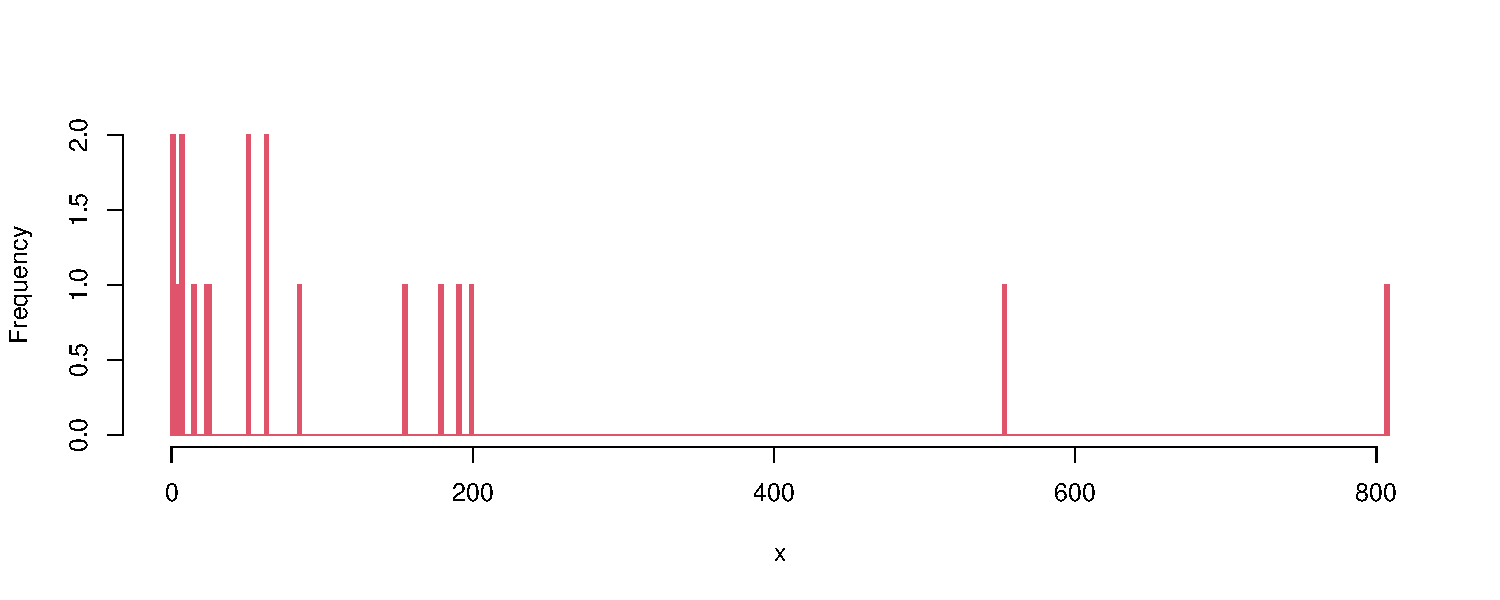
\includegraphics[width=.9\linewidth]{figure/histx-1} 

}


\end{knitrout}
\vspace{-1em}
}
		\item a rough boxplot of $x$ \soln{(Vertical is ok too!  0 pts if axis is not approximately numbered)
\vspace{-2em}
\begin{knitrout}
\definecolor{shadecolor}{rgb}{0.969, 0.969, 0.969}\color{fgcolor}

{\centering 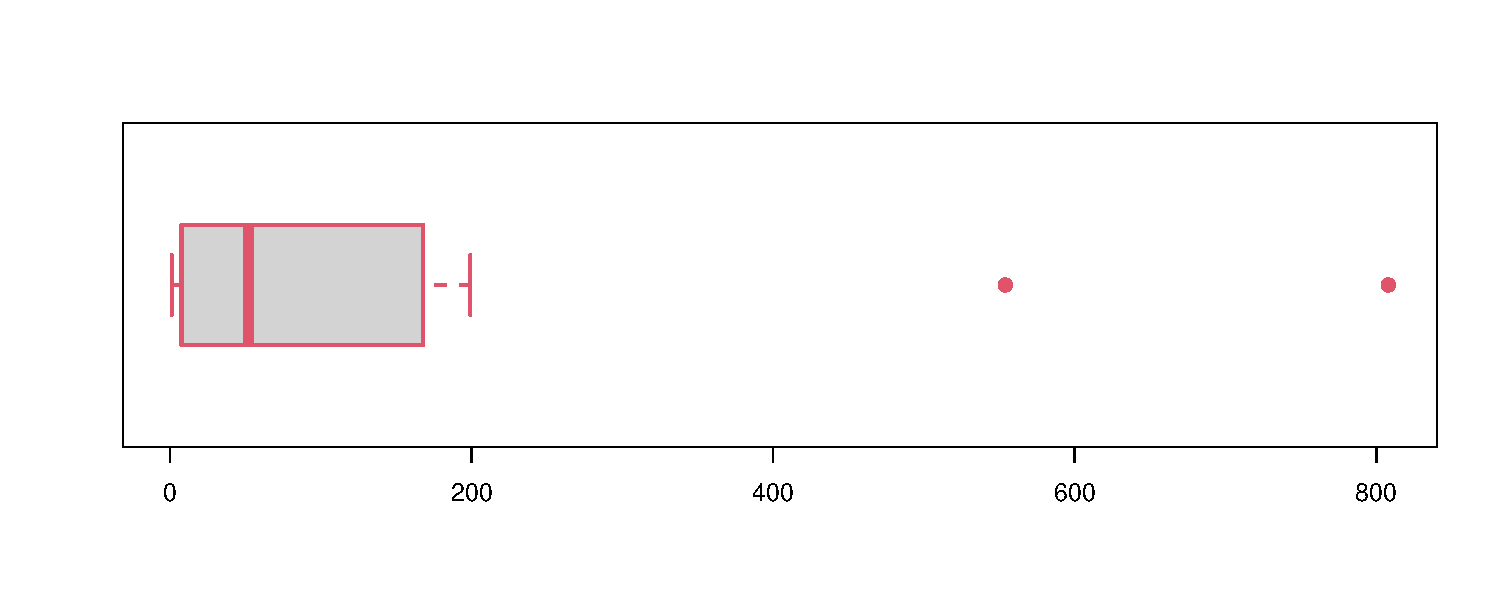
\includegraphics[width=.9\linewidth]{figure/boxpx-1} 

}


\end{knitrout}
\vspace{-2em}}
\end{itemize}
and describe the shape of the distribution in words.
\soln{\\The distribution of the data is heavily skewed to the right.}
\vspace{1ex}
}
%\ifthenelse{\boolean{wSoln}}{}{\clearpage}

%	\probit[8]{Compute:% 
%\begin{itemize}
%	\item the mean and sample SD of $2x$.\soln{ round(c(mean=mean(2*x),sd=sd(2*x)))}
%	\item the mean and sample SD of $x+10$.\soln{ round(c(mean=mean(x+10),sd=sd(x+10)))}
%	\item the mean and sample SD of $2x+10$.\soln{ round(c(mean=mean(2*x+10),sd=sd(2*x+10)))}
%	\item the mean and sample SD of $2(x+10)$.\soln{ round(c(mean=mean(2*(x+10)),sd=sd(2*(x+10))))}
%	\end{itemize}
%}
	\probit[3]{Suppose we added two additional observations to $x$, both of which were exactly equal to
the mean of $x$ (as obtained in part (a) above). 
\soln{\\
(TA's: please grade this based on the solution given for (a), even if (a) was wrong.  
Ie, answers that are consistent with (a) are correct; inconsistency w/ (a) is \textit{incorrect}.)


